% !TeX spellcheck = en_EN
% !TeX encoding = UTF-8
% !TeX program = xelatex
%----------------------------------------------------------------------------
\chapter{Conclusion}
%----------------------------------------------------------------------------

In this chapter, we present a case study that demonstrates the practical implementation of a crossroad example using a Raspberry Pi. This case study showcases the application of embedded systems and highlights the integration of hardware and software components.

%----------------------------------------------------------------------------
\section{Case Study}
%----------------------------------------------------------------------------

In the Gamma tutorial, a crossroad example is presented for illustrating statechart compositions, model transformations, formal verification on an initially faulty model. The tutorial has a \textit{Controller} that synchronizes the two \textit{TrafficLight} objects, and provides a way to interrupt the normal workflow of the crossroad. The tutorial uses inbound and outbound ports to represent the interaction points of the system with its environment, the aforementioned police interrupt button and 4 event for each lamp component that represents the 3 color (red, yellow, green) plus an extra event where no lamp is on. By applying the C code generator to this tutorial example, we can transform the statechart composition into C code that utilizes the specified inbound and outbound ports to transfer these events to a physical form, utilizing a custom hardware board.

\begin{figure}[h]
	\centering
	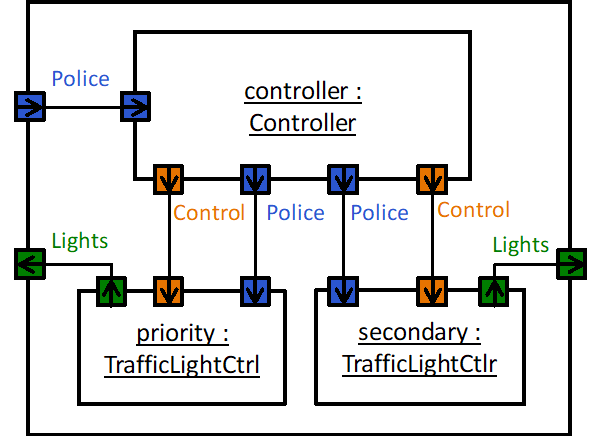
\includegraphics[width=0.6\textwidth]{images/crossroad-component.png}
	\caption{The overview of the crossroad component.}
	\label{fig:crossroad}
\end{figure}

The hardware configuration, acting as a hat for the Raspberry Pi, expands its functionality to act as a crossroad system. The crossroad hardware comprises two red LEDs, two yellow LEDs, and two green LEDs, representing the traffic lights, as well as a button that serves as police interrupt signal.

\begin{figure}[h]
	\centering
	\rotatebox{90}{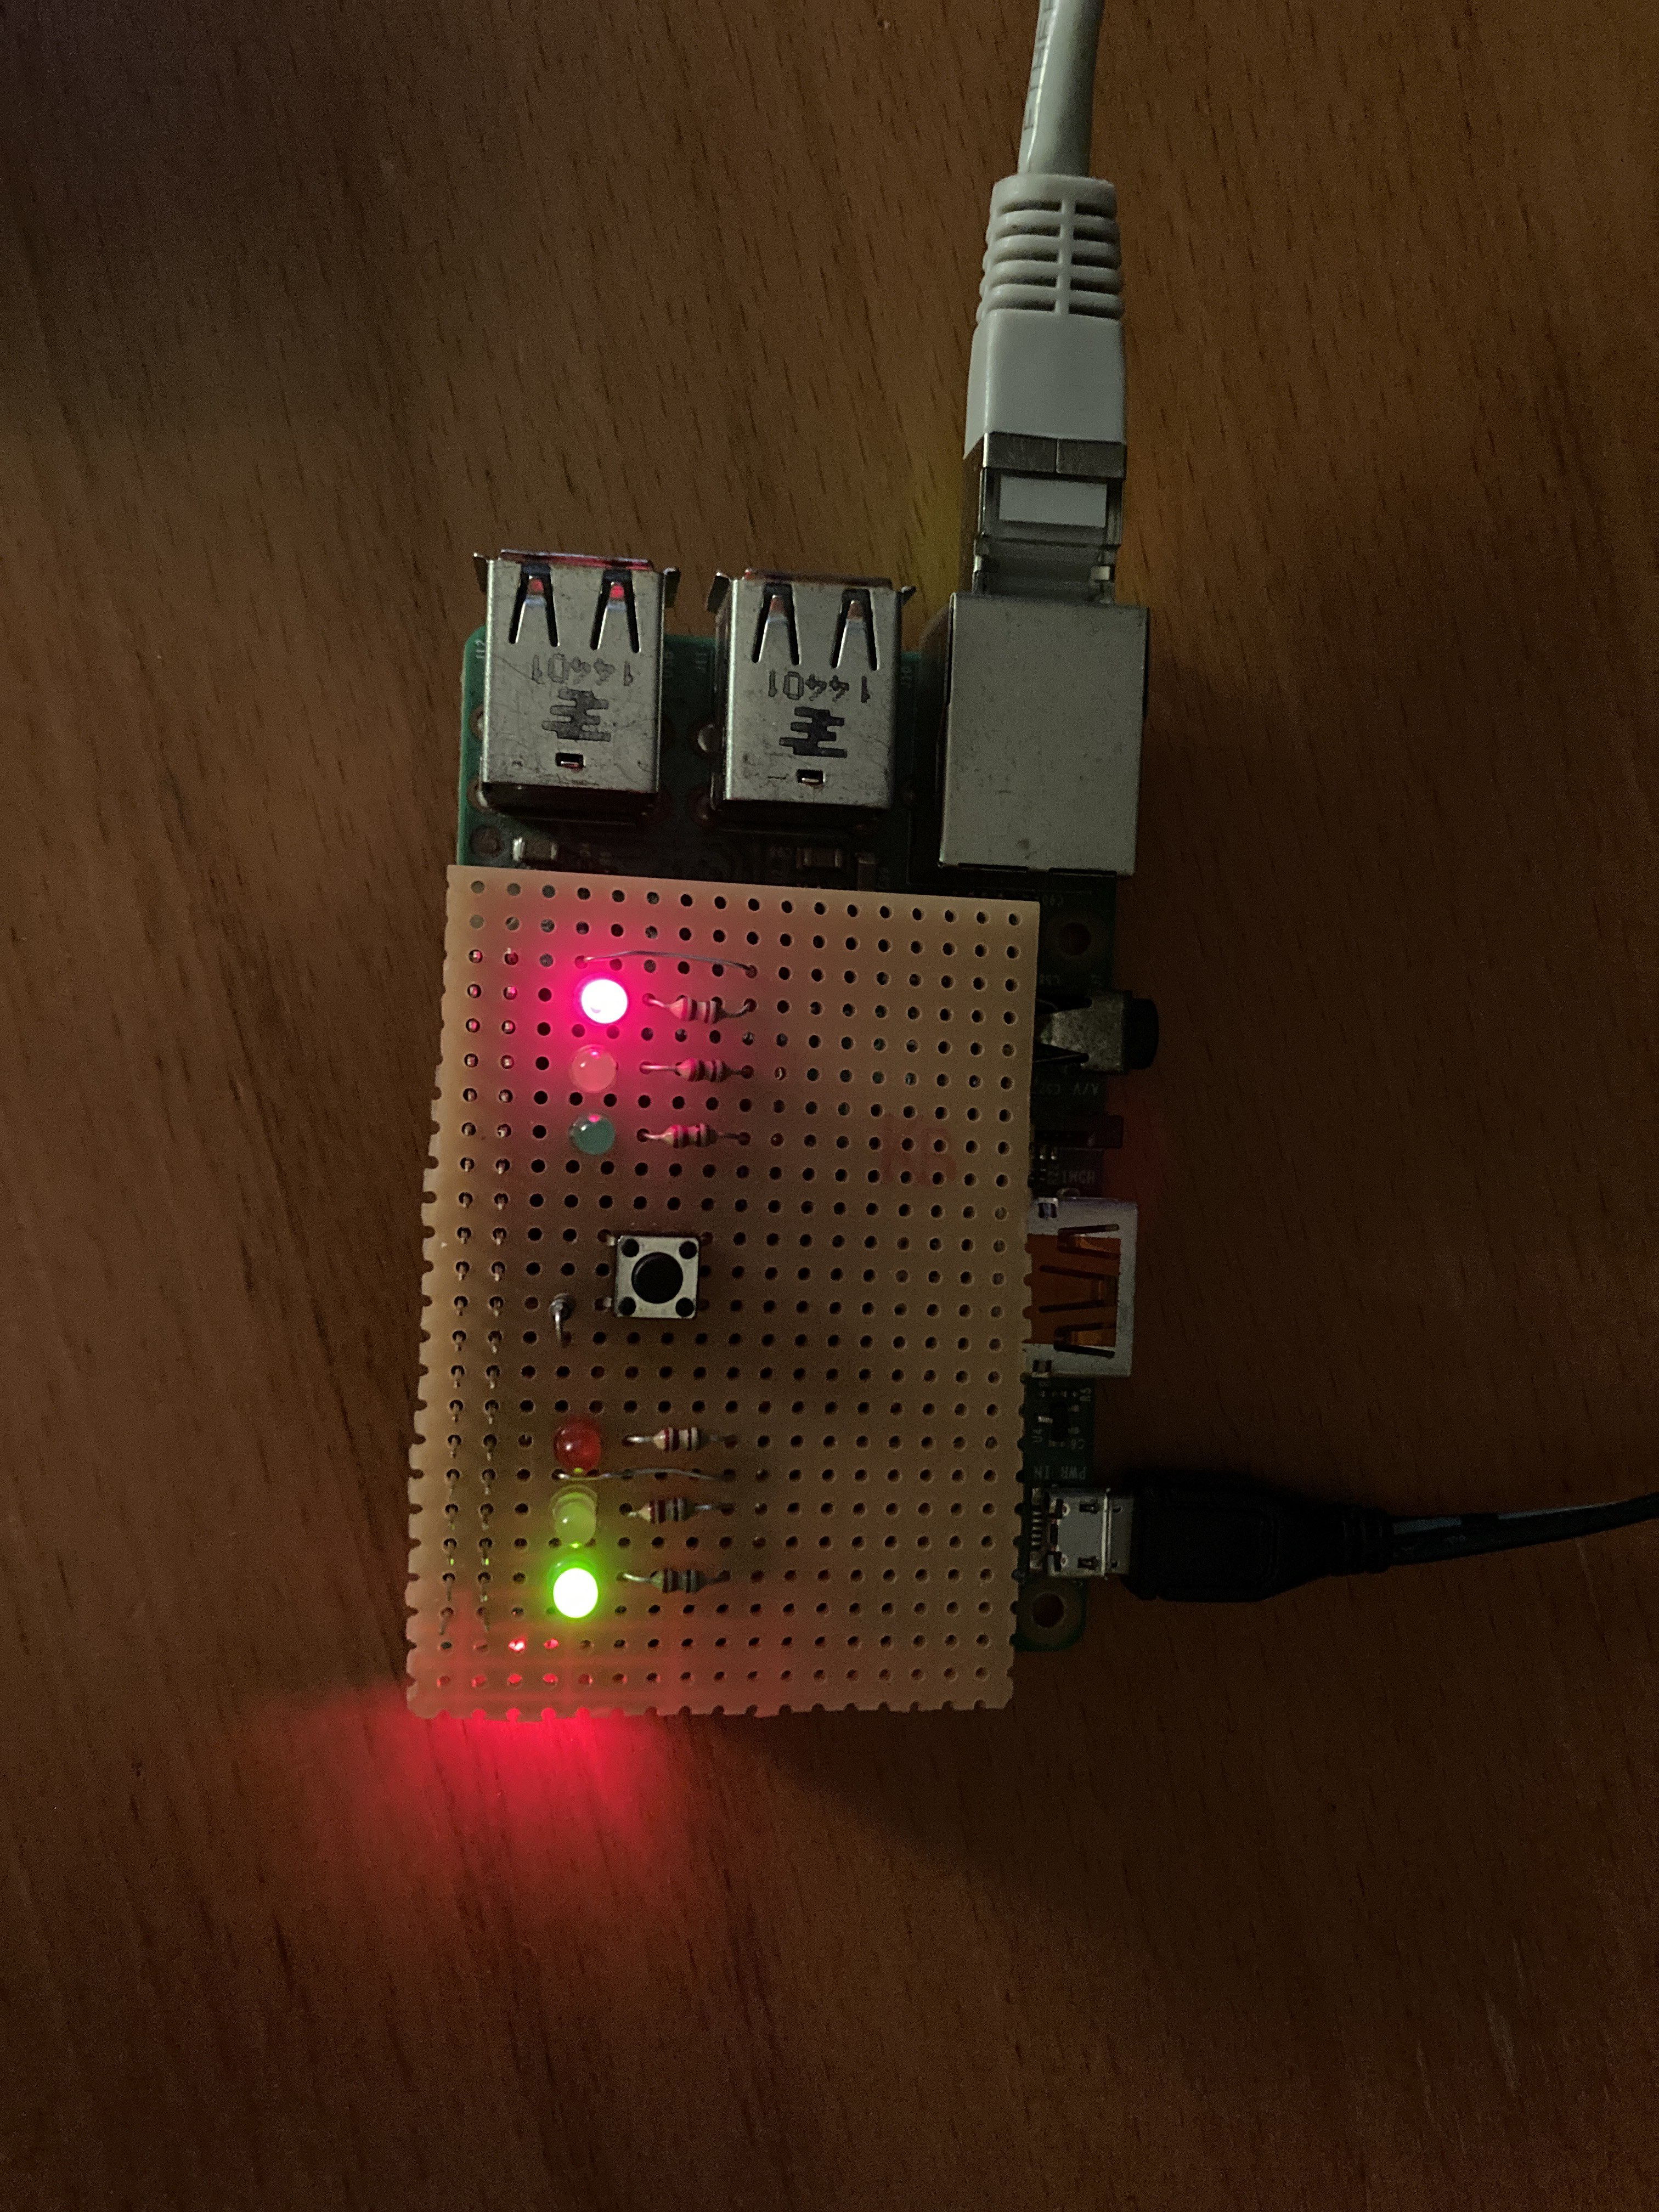
\includegraphics[width=0.6\textwidth]{images/normal-crossroad.png}}
	\caption{The code deployed on a Raspberry Pi.}
	\label{fig:raspberry}
\end{figure}

After generating the C code from the Gamma tutorial's crossroad example, I found that the generated code worked seamlessly in controlling the simulated crossroad system. However, to fully drive the model and observe its behavior, I had to create an additional file that acted as the driver. This driver source file was responsible for reading the output events generated by the model and setting the input events, which in this case were triggered by a button. The button input was detected by monitoring its rising edges, and the corresponding output events were used to control the behavior of the LEDs. By developing this module, I was able to establish a complete interaction loop between the simulated crossroad system and its environment, enabling me to observe the desired outputs reflected through the LEDs based on the input events triggered by the button. This additional file served as a bridge between the generated code and the hardware components, ensuring the seamless integration and functionality of the model in a practical setting.

%----------------------------------------------------------------------------
\section{Overview}
%----------------------------------------------------------------------------

This case study provides an overview of the successful generation and compilation of code from the Gamma tutorial's crossroad example onto a Unix platform, specifically the Raspberry Pi. One of the key highlights of this case study is the ease with which the generated code was compiled without encountering any errors or warnings. This case study underscores the practicality and efficiency of using the Gamma framework and its code generator module for developing embedded systems software.
